% ---------------------------------------------------------------------------- %
\subsection{Aufbau}
% ---------------------------------------------------------------------------- %

Das System besteht  aus zwei Teilen. Aus Sensoren, welche sich  direkt bei den
einzelnen Solarmodulen  befinden und einer Zentrale,  welche die Informationen
der Sensoren auswertet.

\begin{figure}[h!]
    \centering
    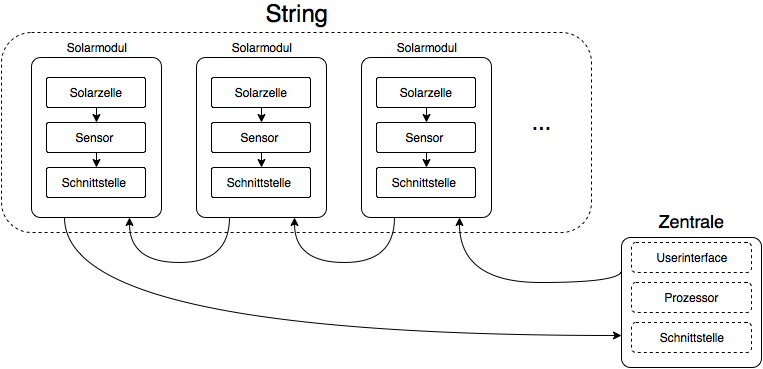
\includegraphics[width=.9\textwidth]{images/blockdiag.png}
    \caption{Blockdiagramm Hardwareaufbau}
    \label{fig:blockdiag:hardware}
\end{figure}


% TODO
% ---------------------------------------------------------------------------- %
\subsection{Spezifikationen}
% ---------------------------------------------------------------------------- %


% ---------------------------------------------------------------------------- %
\subsubsection{Sensor}
% ---------------------------------------------------------------------------- %

Der Sensor besteht  aus einer m\"oglichst kleinen  Leiterplatte, welche direkt
bei den  einzelnen Modulen installiert  werden kann. Die Gr\"osse  des Sensors
sollte maximal 5cm auf 5cm betragen.

Der Energiebedarf des  Sensor wird maximal 200mW betragen  wobei eine Leistung
von unter 100 mW angestrebt wird

Jeder  Sensor  \"uberwacht  dabei  die   Spannung  der  jeweiligen  Zelle  und
\"ubermittelt diese  in regelm\"assigen  Zeitabst\"anden an  die Zentrale. Die
Spannungsmessung und  die Kommunikation  werden von einem  Energiesparenden 32
Bit Mikrokontroller geregelt.

F\"ur  die  Daten\"ubertragung   werden  keine  zus\"atzlichen  Installationen
ben\"otigt. Die Kommunikation findet \"uber die Stromleitungen der Solaranlage
statt. Daf\"ur ist  eine Modulation vorgesehen. F\"ur die  Realisierung werden
folgende zwei M\"oglichkeiten evaluiert:

\begin{itemize}
    \item
        Kapazitiv eingekoppelte Frequenzumtastung (FSK)
    \item
        Serielle \"Ubertragung durch kurzzeitiges Kurzschliessen der Zelle.
\end{itemize}

Die Reichweite des Bussystems sollte minimal 100 Meter Betragen.


% ---------------------------------------------------------------------------- %
\subsubsection{Master-Ger\"at}
% ---------------------------------------------------------------------------- %

\textbf{TODO}
